\chapter{A data-driven background estimate}\label{chap:data_driven}
We identified three sources of backgrounds
(page~\pageref{page:background_categories}). The backgrounds from charge
misidentification and from non-prompt leptons are analysed with data driven
techniques.
\section{Charge misidentification}\label{sec:charge_misid}
Standard Model processes with prompt leptons of opposite charge are very
common at the LHC. They can contribute to the top partners background if the
charge of one of the leptons is incorrectly measured.
For muons in the \pt range considered in this analysis, the charge
misidenfication rate is extremely small ($\approx10^{-5}$) and their contribution to the background is
negligible~\cite{susy2011}. The magnitude of this contribution due to electrons can be derived from the data by using the \Z boson resonance. 
The fraction of misidentified leptons is obtained by considering events with two electrons in which the invariant mass of the leptons falls inside the 
\Z boson mass window: $\unit[76]{GeV}< M(\Lep \Lep) <\unit[106]{GeV}$. These events must pass all cleaning and trigger requirements and the electrons are likewise required to pass all 
quality cuts, but the selection based on the number of jets. As can be seen in the tables~\ref{tab:ZWindowBkgd} and~\ref{tab:ZWindowSig}, this sample is expected to be completely dominated by $\Z$+jets.

\begin{table}[htb]
    \centering
\begin{tabular}{*9c}
    \toprule
                & total & \ttbar    & $\Z$+jets & $\W$+jets & $\W\Z$ & $\Z\Z$ & \ttbar$\W$ & \ttbar$\Z$   \\
                \midrule
                in $\Z$ window & 9.3$\cdot 10^{5}$      & 644       & 9.3$\cdot 10^{5}$      &  35        & 205   &  46.2   & 1.89      & 8.62      \\
 same-sign      & 1090         & 1.84      & 1050       & 9.97      & 8.9   &  1.02   & 0.62      & 0.20      \\
 \bottomrule
\end{tabular}
\caption{Expected event yields within the \Z invariant mass window ($\unit[76]{GeV}< M(\Lep \Lep) <\unit[106]{GeV}$) for the background contributions. The backgrounds not shown yield negligible
         contributions to this phase space region.}
\label{tab:ZWindowBkgd}
\end{table}

\begin{table}[htb]
    \centering
\begin{tabular}{*9c}
    \toprule
$T_{5/3}$ mass [GeV]  & 400       & 450       & 500       & 550       & 600       & 650       & 700       & 750       \\ 
\midrule
 in \Z window         & 22.6      & 9.84      & 4.04      & 1.81      & 0.928     & 0.464     & 0.224     & 0.123     \\ 
 same-sign           & 12.1      & 4.74      & 1.79      & 0.716     & 0.359     & 0.145     & 0.075     & 0.0345    \\ 
 \bottomrule
\end{tabular}
\caption{Expected event yields within the \Z invariant mass window
    ($\unit[76]{GeV}< M(\Lep \Lep) <\unit[106]{GeV}$) for the eight \TP signal  points.}
\label{tab:ZWindowSig}
\end{table}


Applying the same method to data we obtain $858330$ events in the \Z mass
window; $1014$ events remain upon applying the same-sign requirement. The probability of misidentifying the charge of each 
lepton is computed by assuming that the entirety of the same-sign contribution is due to misidentified \Z+jets events and is found to be $5.89 \times 10^{-4}$. To confirm that this upper limit is close to the true probability, we consider the dilepton invariant mass spectrum shown in Figure~\ref{fig:ZWindowMassPeak}. Both 
the simulation and the mass spectrum suggest that the upper limit is close
to the true probability (within approximately 1\% according to the
simulation). We note that this  estimated charge misidentification
probability is consistent with the measurement in~\cite{susy2011}.

\begin{figure}[htb]
\centering
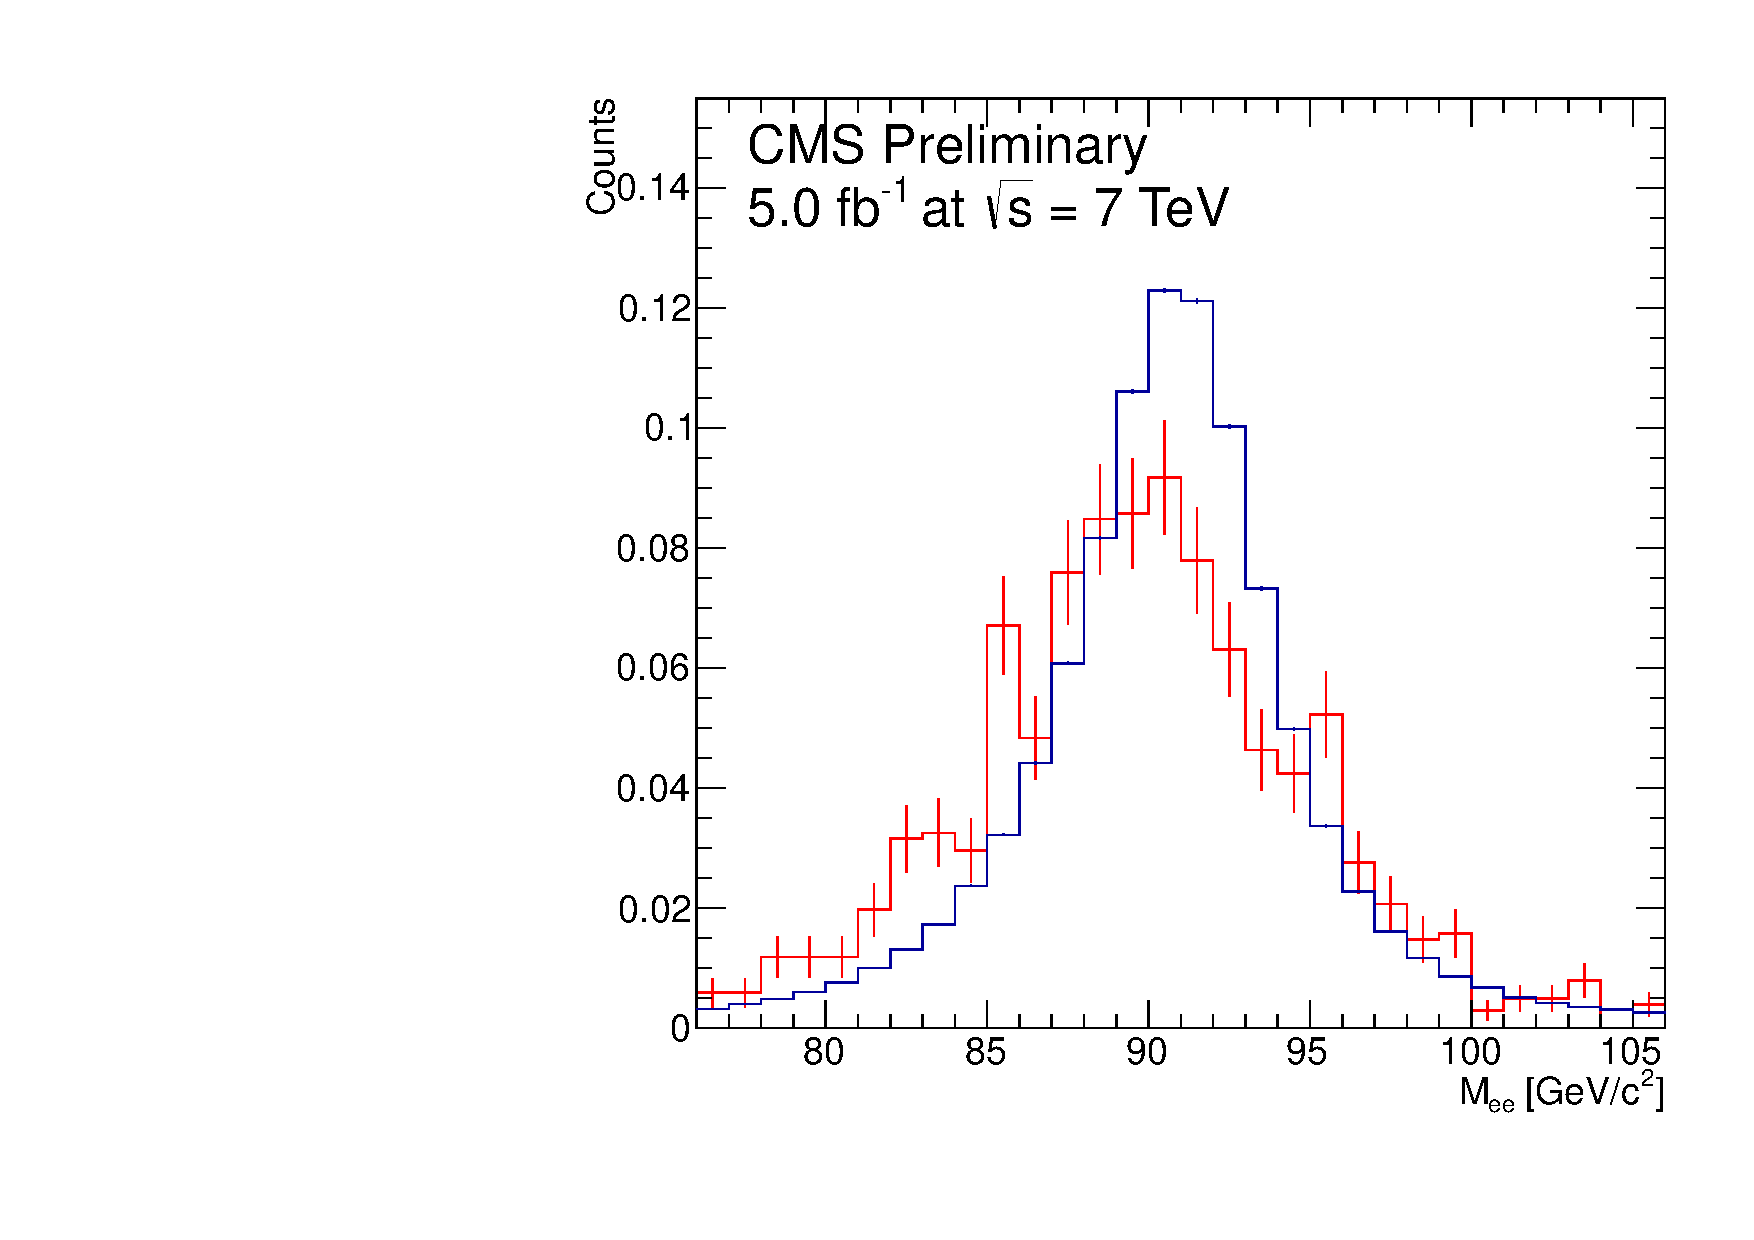
\includegraphics[width=.7\textwidth]{images/pdf/ChargeMisID_ZMass.pdf}
\caption{The dilepton invariant mass spectrum for electrons in data. The opposite-sign distributions are shown in blue and 
the same-sign ones are in red. Both distributions are normalized to unit area.}
\label{fig:ZWindowMassPeak}
\end{figure}

The number of expected same-sign events due to charge misidentification is estimated by considering the total number of events passing the 
full selection, but having oppositely charged leptons. These events are
multiplied by
the charge misidentification probability.

\section{Same-sign non-prompt background}
Non-prompt leptons are the result of the decays of heavy flavour quarks,
decays in flight or conversions. The description of this background in the
Monte Carlo samples is unsatisfactory, and a data-driven estimate is needed.

The so called \emph{tight-loose} method is employed. 
The goal of this method is to measure the probability of a non-prompt lepton
passing the analysis selection~(\ref{sec:fake_rate}) and then to calculate the expected number of
events contaminating our final sample by using this
probability~(\ref{sec:fake_prediction}).

\subsection{Measuring the tight-to-loose ratio}\label{sec:fake_rate}
This method defines two
types of leptons: a \emph{tight} lepton, which is exactly the same as
in~\ref{sec:muon_selection} and~\ref{sec:electron_selection}, and a
\emph{loose} lepton, whose selection criteria are relaxed as follows:
\begin{description}
    \item[loose electron]\hspace*{\fill}\\
        \begin{itemize}
            \item no transverse impact parameter requirements
            \item no conversion rejection
            \item relative isolation relaxed from 0.15 to 0.60
        \end{itemize}
    \item[loose muon]\hspace*{\fill}\\ 
        \begin{itemize}
            \item transverse impact parameter relaxed from
                \unit[0.02]{cm} to \unit[2]{cm}
            \item relative isolation relaxed from 0.20 to 0.40
            \item no requirements on the number of hits in the tracker, nor
                on the number of muon chambers with matching segments
            \item normalized $\chi^2 < 50$ instead of 10
        \end{itemize}
\end{description}
These selections are studied to include \eg leptons from heavy flavour
hadrons: they are usually close to a jet, hence not isolated, and they also
have a larger impact parameter, as the hadron decays on a much larger
timescale with respect to a \TP or a top quark.
Conversion electrons also have to be taken into account, so that the
requirement against conversion rejection has to be eliminated as well.

The relevant quantity is the tight-to-loose ratio, representing the
probability that a non-prompt lepton is identified as tight:
\begin{equation*}
    f = \dfrac{\text{number of tight leptons}}{\text{number of loose
    leptons}}
\end{equation*}
However, this ratio is close to the probability for a non-prompt lepton to
pass the tight selection only if it is calculated on a sample where the
prompt component is negligible. Such a sample can be built from the
\texttt{SingleMu} and \texttt{DoubleElectron} primary datasets by enforcing
cuts aiming to reject leptons from \W and \Z bosons:
\begin{itemize}
    \item exactly one loose lepton in each event
    \item at least one jet with $\pt > \unit[40]{GeV}$ and $\Delta R > 1$
        relative to the lepton
    \item $\met < \unit[25]{GeV}$
    \item $\mt < \unit[25]{GeV}$
    \item extended \Z veto: reject the event if the invariant mass of the
        lepton and any jet is in the \unit[76-106]{GeV} window
\end{itemize}
The \met and \mt selections are meant to exclude the presence of \W bosons,
and the \Z veto now includes all the jets, as a second lepton can be incorrectly
identified as a jet.

Even with this selection, the contamination from prompt leptons is still
fairly large. This can be estimated from the Monte Carlo $\Wjets$ and
$\Zjets$ samples. The results are shown in
tables~\ref{tab:FRwMCEl} and~\ref{tab:FRwMCMu}.
\begin{table}[htb]
\begin{center}
\begin{tabular}{*4c}
    \toprule
 & 	 loose & 	 tight & 	 ratio \\
 \midrule
 $\Wjets$ & 	31.6 $\pm$ 0.21 & 	29.3 $\pm$ 0.20 & 	     -     \\
$\Zjets$ & 	21.9 $\pm$ 0.08 & 	20.4 $\pm$ 0.08 & 	     -     \\
$\ttbar$ & 	 0.7 $\pm$ 0.01 & 	 0.6 $\pm$ 0.01 & 	     -     \\
\midrule
Data & 	 1974 & 	  274 & 	0.138 $\pm$ 0.009 \\
Data-MC &	1919.8 $\pm$ 44.43 & 	223.7 $\pm$ 16.55 & 	0.117 $\pm$ 0.009 \\
\bottomrule
\end{tabular}
\caption{Tight to loose ratio for electrons in the data and in the MC. The line
    Data-MC subtracts from the data the prompt lepton contribution due to
    $\Wjets$, 
$\Zjets$ and $\ttbar$ from the data.}
\label{tab:FRwMCEl}
\end{center}
\end{table}

\begin{table}[htb]
\begin{center}
\begin{tabular}{*4c}
    \toprule
 & 	 loose & 	 tight & 	 ratio \\
 \midrule
$\Wjets$ & 	4505.0 $\pm$ 26.36 & 	4374.8 $\pm$ 25.97 & 	     -     \\
$\Zjets$ & 	604.0 $\pm$ 4.36 & 	585.8 $\pm$ 4.29 & 	     -     \\
$\ttbar$ & 	85.5 $\pm$ 1.20 & 	80.4 $\pm$ 1.16 & 	     -     \\
\bottomrule
Data & 	33770 & 	12170 & 	0.360 $\pm$ 0.004 \\
Data-MC &	28575.5 $\pm$ 185.70 & 	7129.1 $\pm$ 113.42 & 	0.249 $\pm$ 0.004 \\
\bottomrule
\end{tabular}
\caption{Tight to loose ratio for muons in the data and in the MC. The line
    Data-MC subtracts from the data the prompt lepton contribution due to
    $\Wjets$, 
$\Zjets$ and $\ttbar$ from the data.}
\label{tab:FRwMCMu}
\end{center}
\end{table}

In order to avoid being directly dependent on the MC, we note that the
contamination from prompt leptons is negligible if we restrict the \pt range
of the leptons to $\unit[25]{GeV} < \pt < \unit[35]{GeV}$. The overlap of
this \pt range with that of the signal selection in the analysis ($\pt >
\unit[30]{GeV}$) is small, but when the tight-to-loose ratio is corrected
for the contribution of prompt leptons, it becomes nearly independent from
the \pt (see figure~\ref{fig:CorFRvsLepPt}).
\begin{figure}[htb]
    \centering
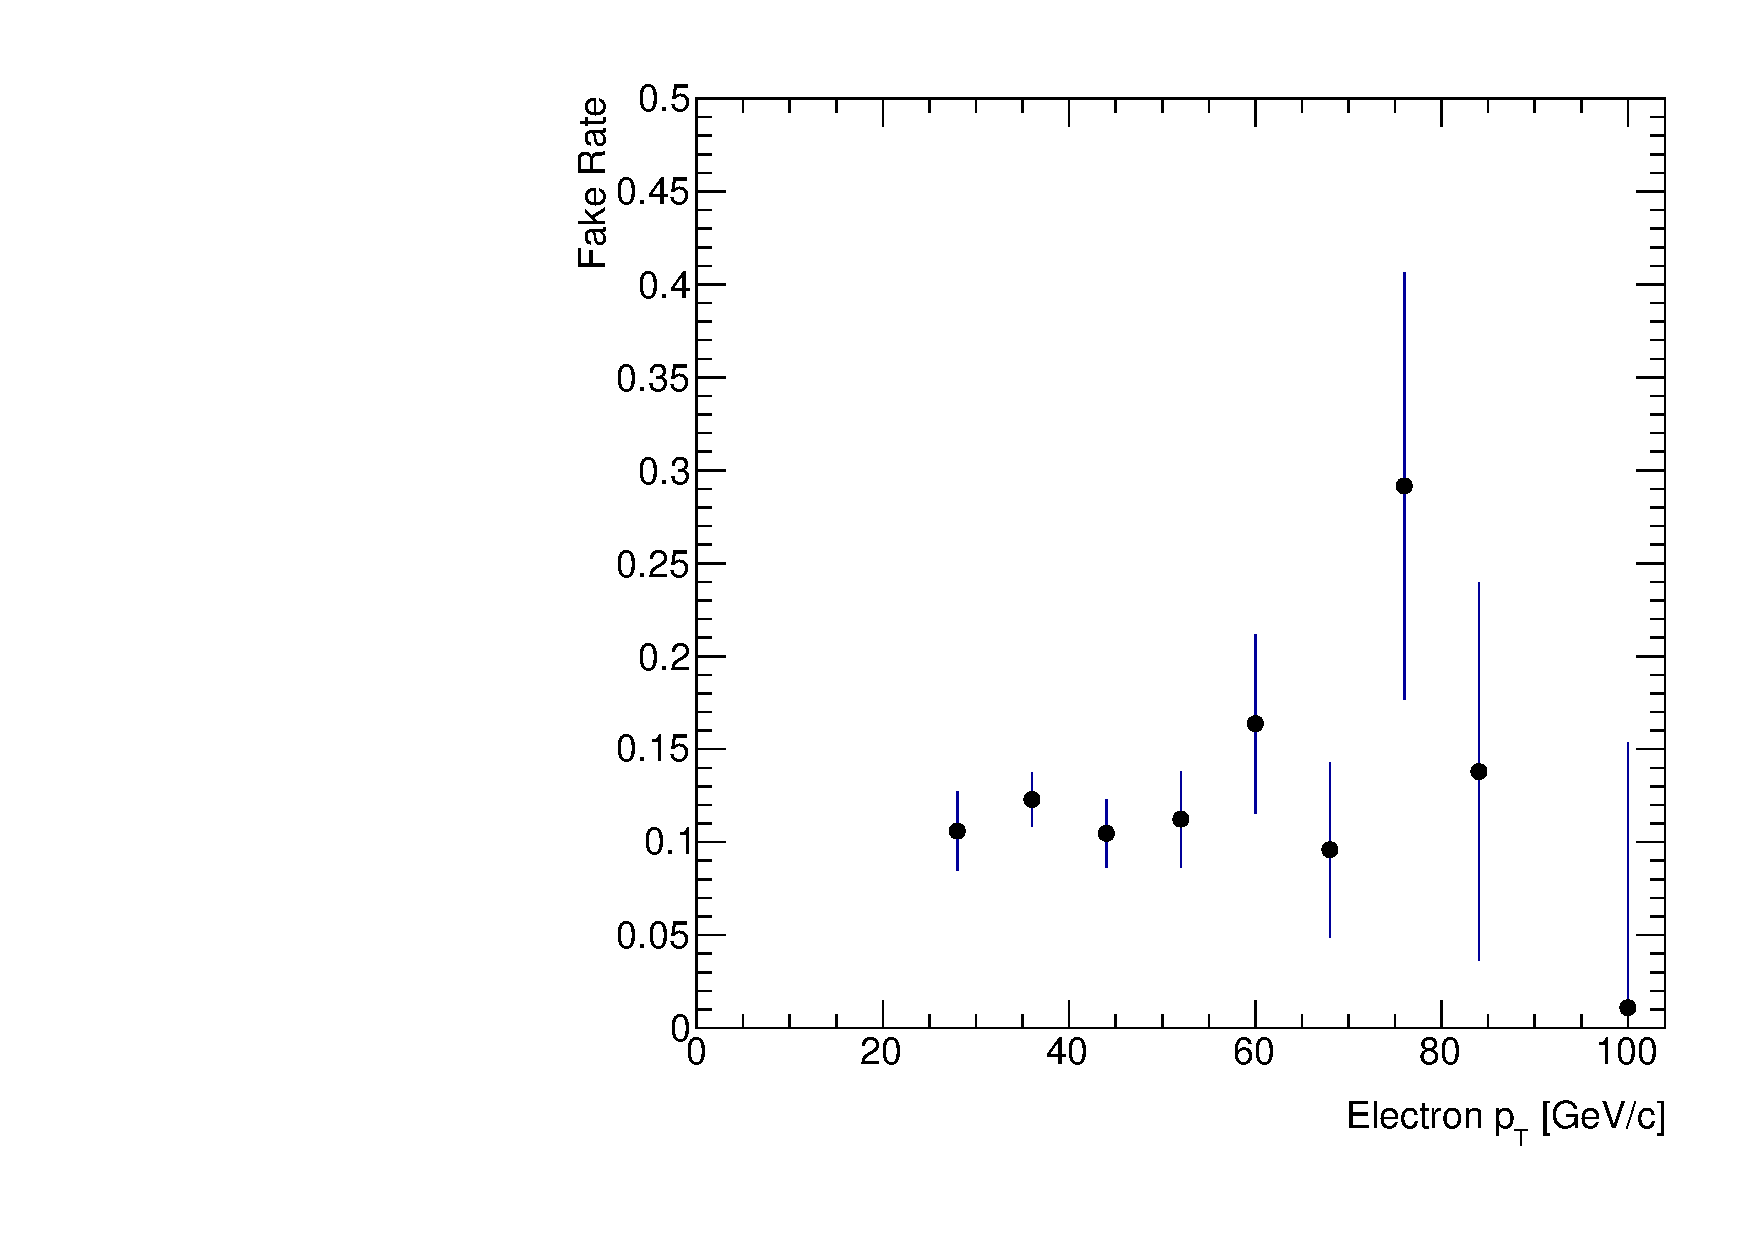
\includegraphics[width=0.7\textwidth]{images/pdf/h_FR_ElPt} \\
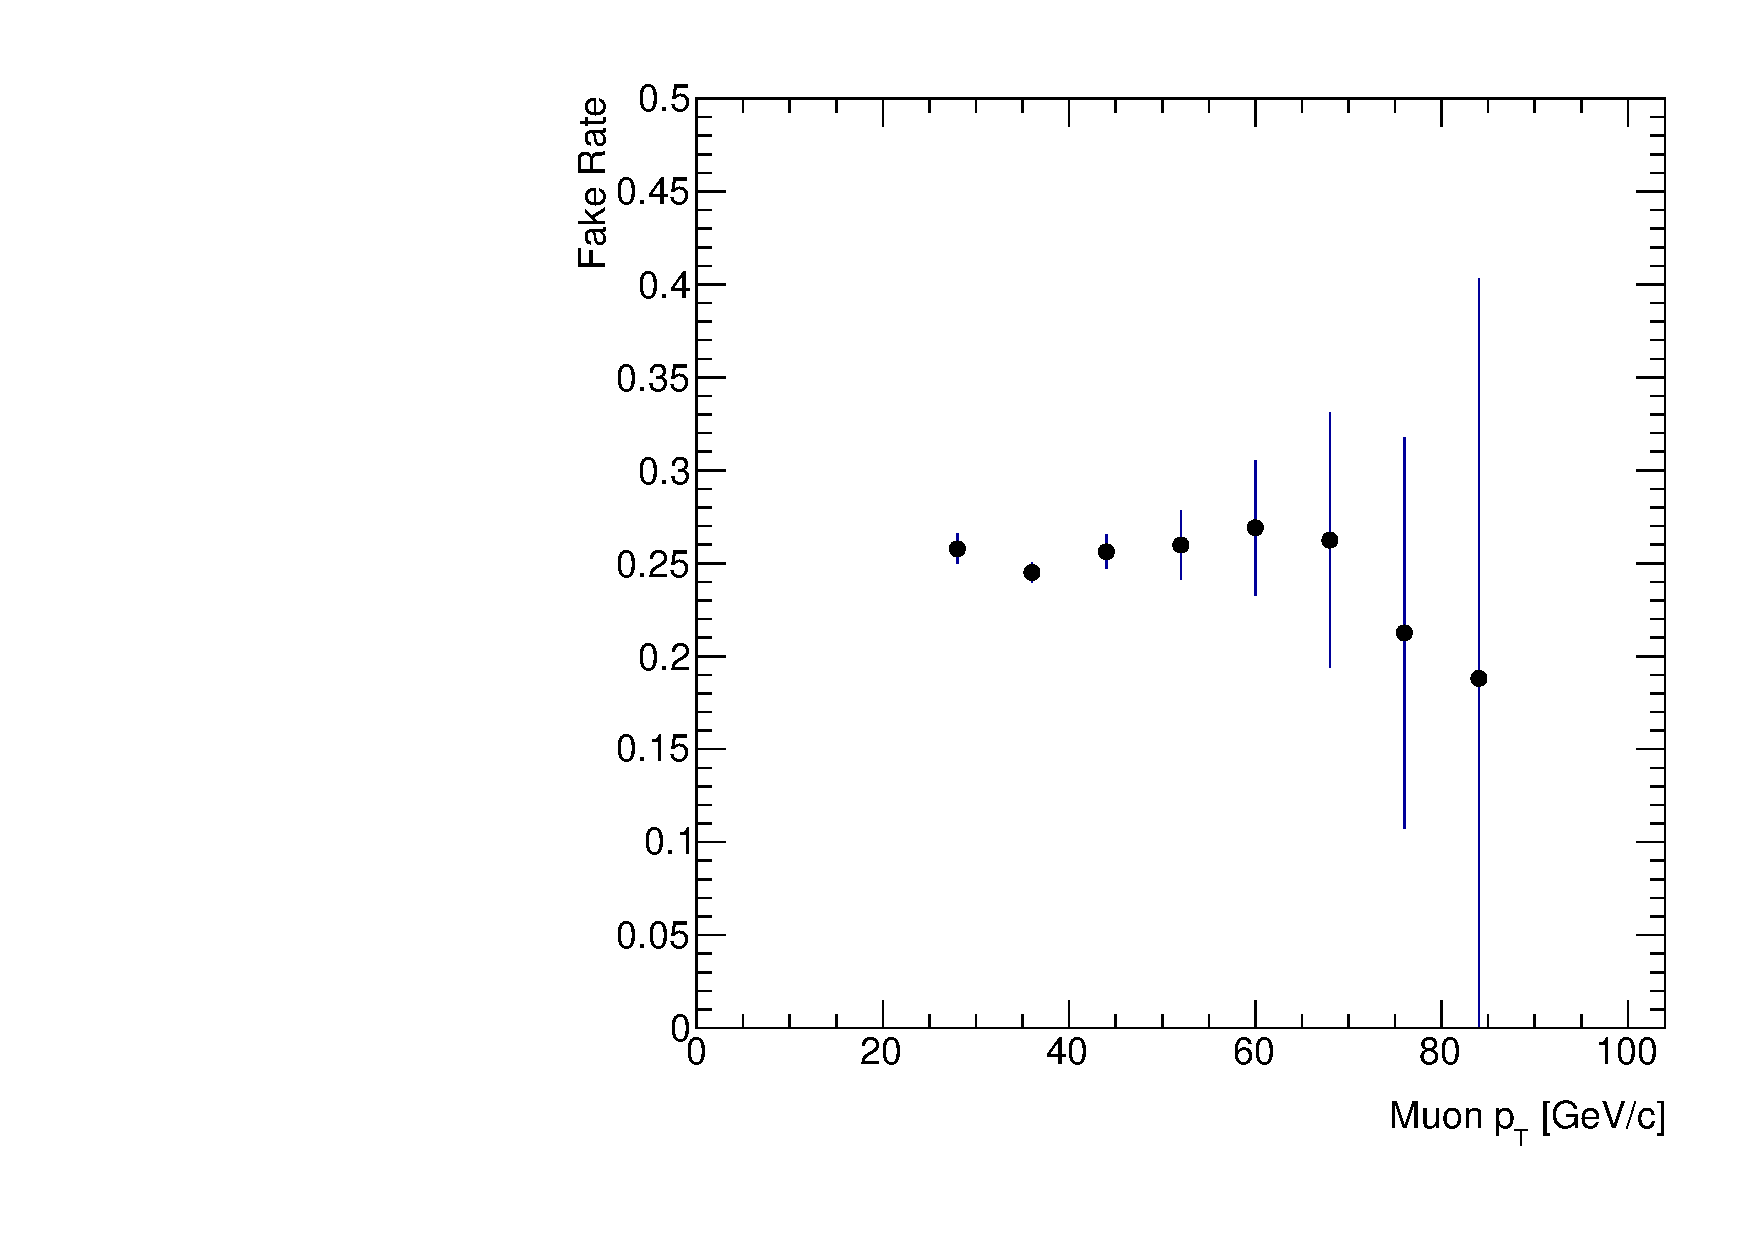
\includegraphics[width=0.7\textwidth]{images/pdf/h_FR_MuPt} 
\caption{The corrected tight-to-loose ratio, loosely speaking the
    \emph{fake rate}, as a function of $\pt$ for electrons (left) and muons (right). The correction is accomplished by subtracting the MC-based 
         $\W$, $\Z$ and $\ttbar$ contributions from the data.}
\label{fig:CorFRvsLepPt}
\end{figure}
\begin{table}[htb]
    \centering
\begin{tabular}{*4c}
    \toprule
 & 	 loose & 	 tight & 	 ratio \\
 \midrule
$\Wjets$ & 	 7.0 $\pm$ 0.10 & 	 6.2 $\pm$ 0.09 & 	- \\
$\Zjets$ & 	 8.1 $\pm$ 0.05 & 	 7.2 $\pm$ 0.05 & 	- \\
$\ttbar$ & 	 0.1 $\pm$ 0.00 & 	 0.1 $\pm$ 0.00 & 	- \\
\midrule
Data & 	 1698 & 	  191 & 	0.112 $\pm$ 0.009 \\
Data-MC &	1682.9 $\pm$ 41.21 & 	177.5 $\pm$ 13.82 & 	0.105 $\pm$ 0.009 \\
\bottomrule
\end{tabular}
\caption{Tight to loose ratio for electrons in the data and in the MC with
    the $\pt$ range of
    the electron restricted to the 25-\unit[35]{GeV} range.
The line Data-MC subtracts the prompt lepton contribution due to $\Wjets$,
$\Zjets$ and $\ttbar$ from the data.}
\label{tab:FRwMCEl_Pt2535}
\end{table}


\begin{table}[htb]
    \centering
\begin{tabular}{*4c}
    \toprule
 & 	 loose & 	 tight & 	 ratio \\
 \midrule
$\Wjets$ & 	995.1 $\pm$ 12.37 & 	942.9 $\pm$ 12.03 & 	- \\
$\Zjets$ & 	355.4 $\pm$ 3.33 & 	339.1 $\pm$ 3.25 & 	- \\
$\ttbar$ & 	13.9 $\pm$ 0.48 & 	11.8 $\pm$ 0.45 & 	- \\
\midrule
Data & 	40479 & 	11536 & 	0.285 $\pm$ 0.003 \\
Data-MC &	39114.6 $\pm$ 201.60 & 	10242.2 $\pm$ 108.13 & 	0.261 $\pm$ 0.003 \\
\bottomrule
\end{tabular}
\caption{Tight to loose ratio for muons in the data and in the MC with the
    $\pt$ range of the muon restricted to the 25-\unit[35]{GeV} range. 
The line Data-MC subtracts the prompt lepton contribution due to $\Wjets$,
$\Zjets$ and $\ttbar$ from the data.}
\label{tab:FRwMCMu_Pt2535}
\end{table}

With this \pt restriction, the contributions from prompt leptons in the MC
becomes negligible (tables~\ref{tab:FRwMCEl_Pt2535}
and~\ref{tab:FRwMCMu_Pt2535}), and in the following analysis we use only the values
from the data:
\begin{align*}
    f_\E &= 0.112 \pm 0.009 \text{ stat.}\\
    f_\M &= 0.285 \pm 0.003 \text{ stat.}
\end{align*}

\subsection{Heavy flavour content of the samples}
The samples in which these ratios are measured are selected without any
requirements on the heavy flavour content. However, a large part of the
non-prompt background is expected to arise from semileptonic \ttbar. We
therefore have to check that our prediction is stable with respect to
variations in the flavour content.

The b-tagging algorithm described in~\ref{sec:btagging} is used to enrich
our samples of leptons coming from b quarks. This doesn't change the values
calculated in the previous section, within the statistical uncertainties:
\begin{align*}
    f_\E^{\text{btag}} &= 0.120 \pm 0.009 \text{ (stat.)}\\
    f_\M^{\text{btag}} &= 0.280 \pm 0.003 \text{ (stat.)}
\end{align*}

\subsection{Prompt ratio approximation}
The \emph{prompt ratio} $p$ can also be defined as the probability for
a prompt lepton to pass the tight selection. It can be studied with a tag
and probe method in Drell-Yan events where the invariant mass of the leptons
is within \unit[10]{GeV} of the \Z mass. This gives values close to one for
both electrons ($p_\E = 0.92$) and muons ($p_\M = 0.98$). This efficiency is
confirmed in Monte Carlo \Z and \W studies.

This justifies the approximation in all of the following formulae, where
$p_\E = p_\M = 1$ is assumed.
This allows to simplify the calculation of the non-prompt background, as
well as the treatment of the uncertainties.

\subsection{Calculation of the expected event
yields}\label{sec:fake_prediction}
The measure of the non-prompt rate $f_\Lep$ allows to make a prediction on
the number of events with non-prompt leptons contaminating our final
selection.

The idea of the method is best illustrated in the simpler case of single lepton
events.
The total number of leptons $N_\Lep$ passing the loose criteria is composed
of $N_p$ prompt leptons and $N_f$ non-prompt leptons. These numbers are not
directly measurable but they can be related to the number of leptons where
no lepton ($N_{t0}$) or one lepton $N_{t1}$ passes the tight selection:
\begin{align*}
    N_\Lep &= N_p + N_f = N_{t0} + N_{t1}\\
    N_{t1} &= N_p + fN_f\\
    N_{t0} &= (1 - f) N_f
\end{align*}
These relations can be easily inverted to obtain $N_p$ and $N_f$, and mostly
the number of non-prompt leptons passing the tight selection, which is the
expected number of background events in our final sample:
\begin{equation*}
    N_f^\text{pass} = fN_f = \varepsilon N_{t0}
\end{equation*}
Where we conveniently introduced the notation:
\begin{equation*}
    \varepsilon = \dfrac{f}{1 - f}
\end{equation*}
This shows that the number of non-prompt leptons passing the tight cuts is
expressed as a function of the ones failing the cuts, weighted by
$\varepsilon$.

This approach can be generalized to our case of dilepton events, 
in the hypothesis that the probabilities for the two leptons are independent. We will
first assume that the leptons have the same flavour, \ie they are both
electrons or muons.

Now the total number of events passing the loose cuts is the sum of three
contributions: $N_{pp}$ events with two prompt leptons, $N_{fp}$ events with
one prompt and one non-prompt lepton, $N_{ff}$ with two non-prompt leptons.
Again, these are related to the measurable numbers of events $N_{tx}$ with
 $x = 0$, $1$, $2$ leptons passing the tight cuts, the remaining ones
 failing these cuts.
\begin{align*}
    N &= N_{ff} + N_{fp} + N_{pp} = N_{t0} + N_{t1} + N_{t2}\\
    N_{t0} &= (1 - f)^2 N_{ff}\\
    N_{t1} &= (1 - f) N_{fp} + 2f(1 - f)N_{ff}\\
    N_{t2} &= fN_{fp} + f^2N_{ff}
\end{align*}
The matrix of these linear equations can be inverted, and again with the
same procedure illustrated for the single lepton case, we get the number of
events with one non-prompt and two non-prompt leptons for our final
selection:
\begin{align*}
    N_{fp}^\text{pass} &= \varepsilon N_{t1} - 2 \varepsilon^{2} N_{t0}\\
    N_{ff}^\text{pass} &= \varepsilon^2 N_{t0}
\end{align*}
As in the single lepton case, failing leptons get a weight $\varepsilon$,
prompt passing leptons get a weight $1$.
For the mixed case of $N_{fp}$, in case both leptons fail, each of them is
weighted alternatively by $\varepsilon$, the other by $1$, hence the factor
2. 

Finally these formulae can be extended to include the situation where an
electron and a muon are part of the same configuration.
The notation is now $N_{pp}$, $N_{fp}$, $N_{pf}$ and $N_{ff}$, where the
first subscript refers to the electron, the second one to the muon. The
numbers of events passing and failing the selections is written as
$N_{txy}$, with $x$ giving the number of electrons passing the tight cuts
and $y$ giving the number for muons.

The basic equations are then:
\begin{align*}
    N_{t00} &= (1 - f_\E)(1 - f_\M) N_{ff}\\
    N_{t01} &= (1 - f_\E)N_{fp} + (1 - f_\E)f_\M N_{ff}\\
    N_{t10} &= (1 - f_\M)N_{pf} + (1 - f_\M)f_\E N_{ff}\\
    N_{t11} &= N_{pp} + f_\M N_{pf} + f_\E N_{fp} + f_\E f_\M N_{ff}
\end{align*}
From those, the number for the background expected events can be extracted with the
now familiar technique:
\begin{align*}
    N_{pf}^\text{pass} &= \varepsilon_\M N_{t10} - \varepsilon_\E
    \varepsilon_\M N_{t00}\\
    N_{fp}^\text{pass} &= \varepsilon_\E N_{t01} -
    \varepsilon_\E \varepsilon_\M N_{t00}\\
    N_{ff}^\text{pass} &= \varepsilon_\E \varepsilon_\M N_{t00}
\end{align*}

\subsection{Closure tests}\label{sec:closure}
In order to make sure that the method applied for the non-prompt leptonic
background estimate is sound we have tested it on independent Monte Carlo
samples. The MC generator information provides the real non-prompt
contribution to our selection. This number is what we call the
\emph{observed} number of events for the purposes of this paragraph.

The non-prompt ratio for Monte Carlo events was calculated 
in QCD samples, without the selections on the
\met and $\mt$,  as there are no vector bosons in the QCD Monte Carlo:
\begin{align*}
    f_{\E} &= 0.091 \pm 0.017\\
    f_{\M} &= 0.152 \pm 0.002
\end{align*}
These numbers differ from the values in the data since the MC does not
describe accurately the composition of the non-prompt events.

Monte Carlo events are selected with two same-sign leptons, discarding
events where both leptons are actually prompt, \ie the decay
product of a \W or \Z boson.
Therefore all of the dilepton events we observe after
these selections have at least one non-prompt lepton. The method just
described in~\ref{sec:fake_prediction} predicts a
number of \emph{expected} events.

The results are summarized in Table~\ref{tab:ClosureTestsTable}. The $\ttbar$ studies show that the observed yields differ
from the predicted by -39\% for $\E\E$, -29\% for $\M\M$ and -27\% for
$\E\M$. Based on these studies, we assign a 50\% systematic
uncertainty on the estimation of backgrounds due to fake leptons. This is in agreement with the studies done in 
reference~\cite{Chatrchyan:2011wba}.

\begin{table}
\centering
\begin{tabular}{ccc r@{$\pm$}l}
    \toprule
 sample & event type & observed & \multicolumn{2}{c}{expected}  \\ 
 \midrule
W+jets  & $\E\E$ & 17 & $25.11$ & $6.60$\\ %this is with MC FR 
  & $\M\M$ & 0 & $0.68$ & $ 0.36$\\
  & $\E\M$ & 25 & $30.61$ & $8.15$ \\
  \midrule
$t\bar t$  & $\E\E$ & 43 & $70.04$ & $15.40$  \\ %this is with MC FR
  & $\M\M$ & 33 & $46.45$ & $6.48$ \\ 
  & $\E\M$ & 83 & $114.22$ & $24.53$ \\
  \bottomrule
 \end{tabular}
 \caption{Summary of the closure tests on Monte Carlo samples for events
 with two same-sign leptons. Statistical errors only.} 
 \label{tab:ClosureTestsTable} 
\end{table} 

A comparison between the observed and expected distributions for various
kinematical variables (figures~\ref{fig:jet_pt}, \ref{fig:lep_pt}
and~\ref{fig:masses}) also shows good agreement.

\begin{figure}[htb]
    \centering
    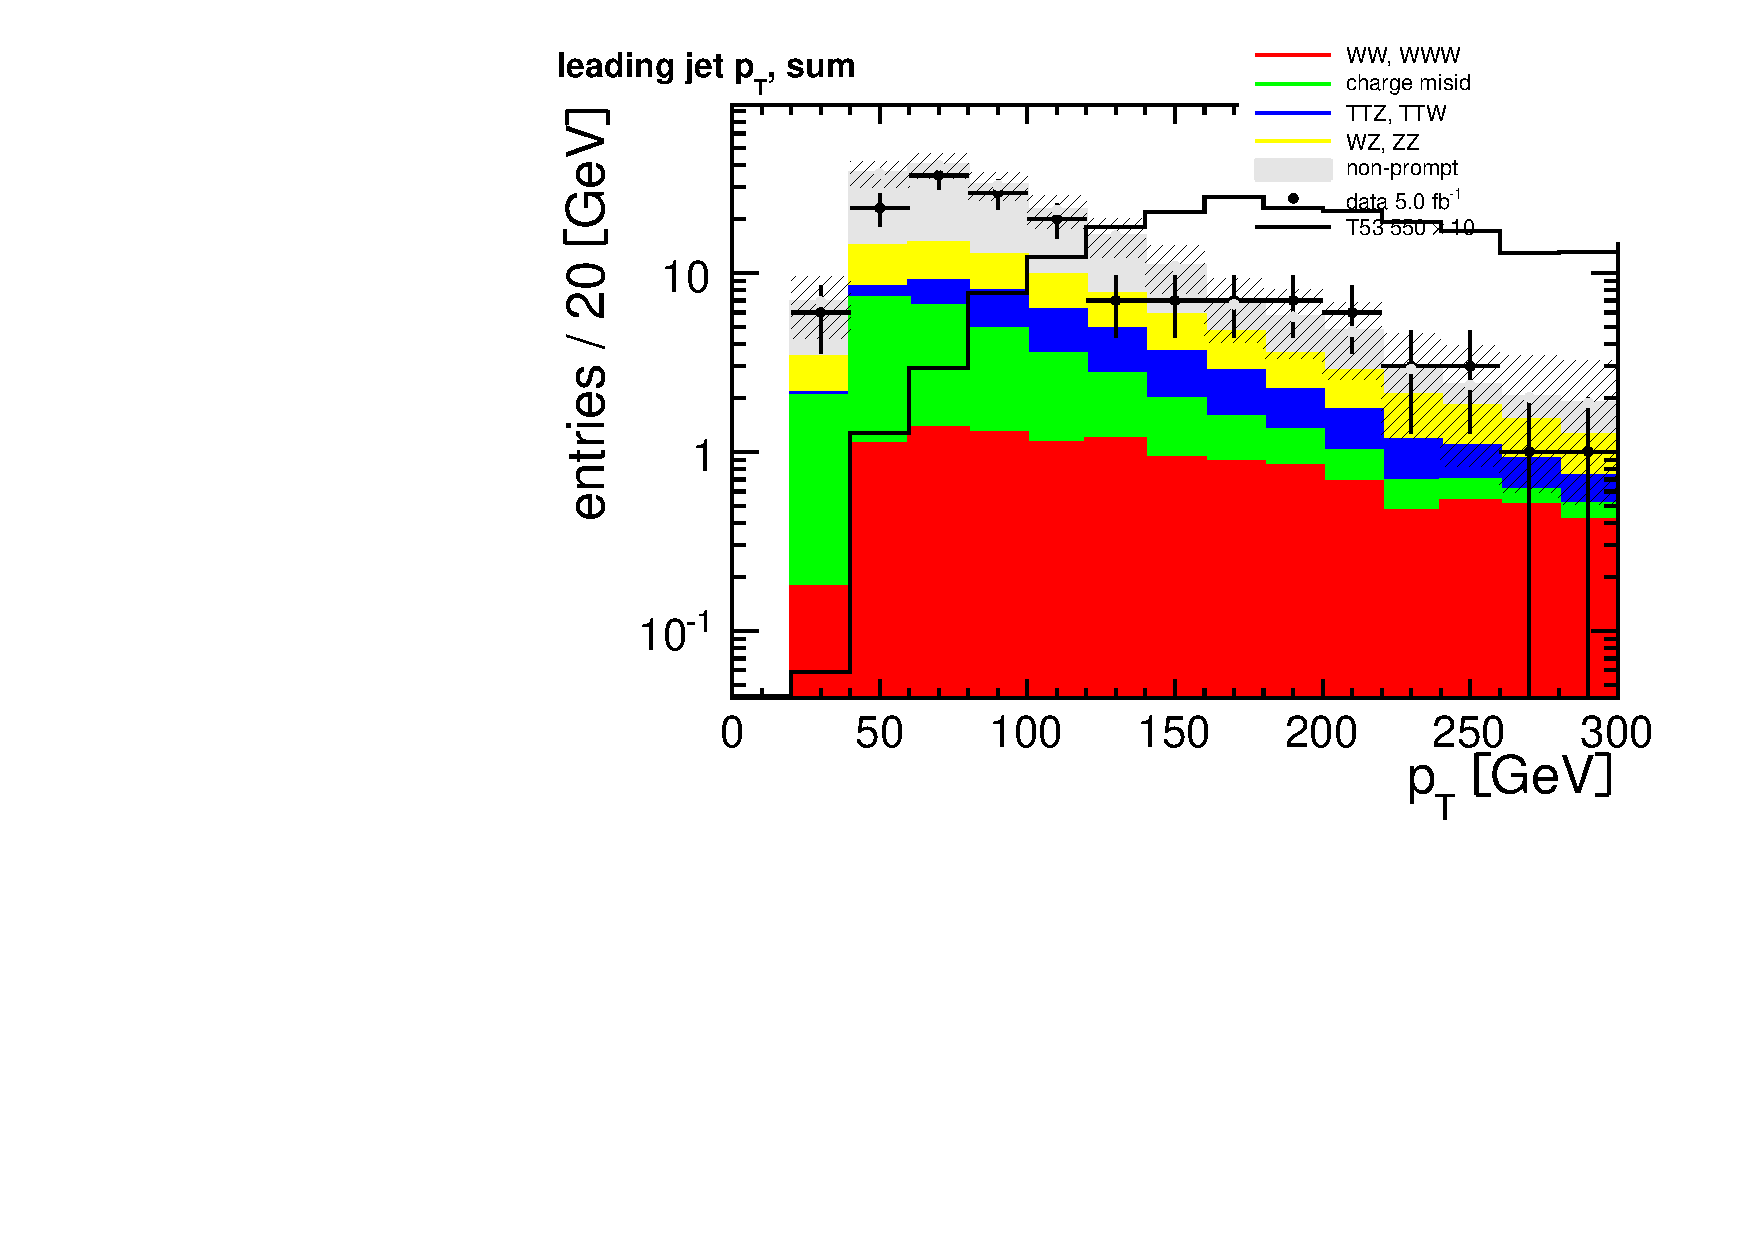
\includegraphics[width=.7\textwidth]{images/pdf/same-sign,_2_jets/jet_pt_1_sum_1}\\
    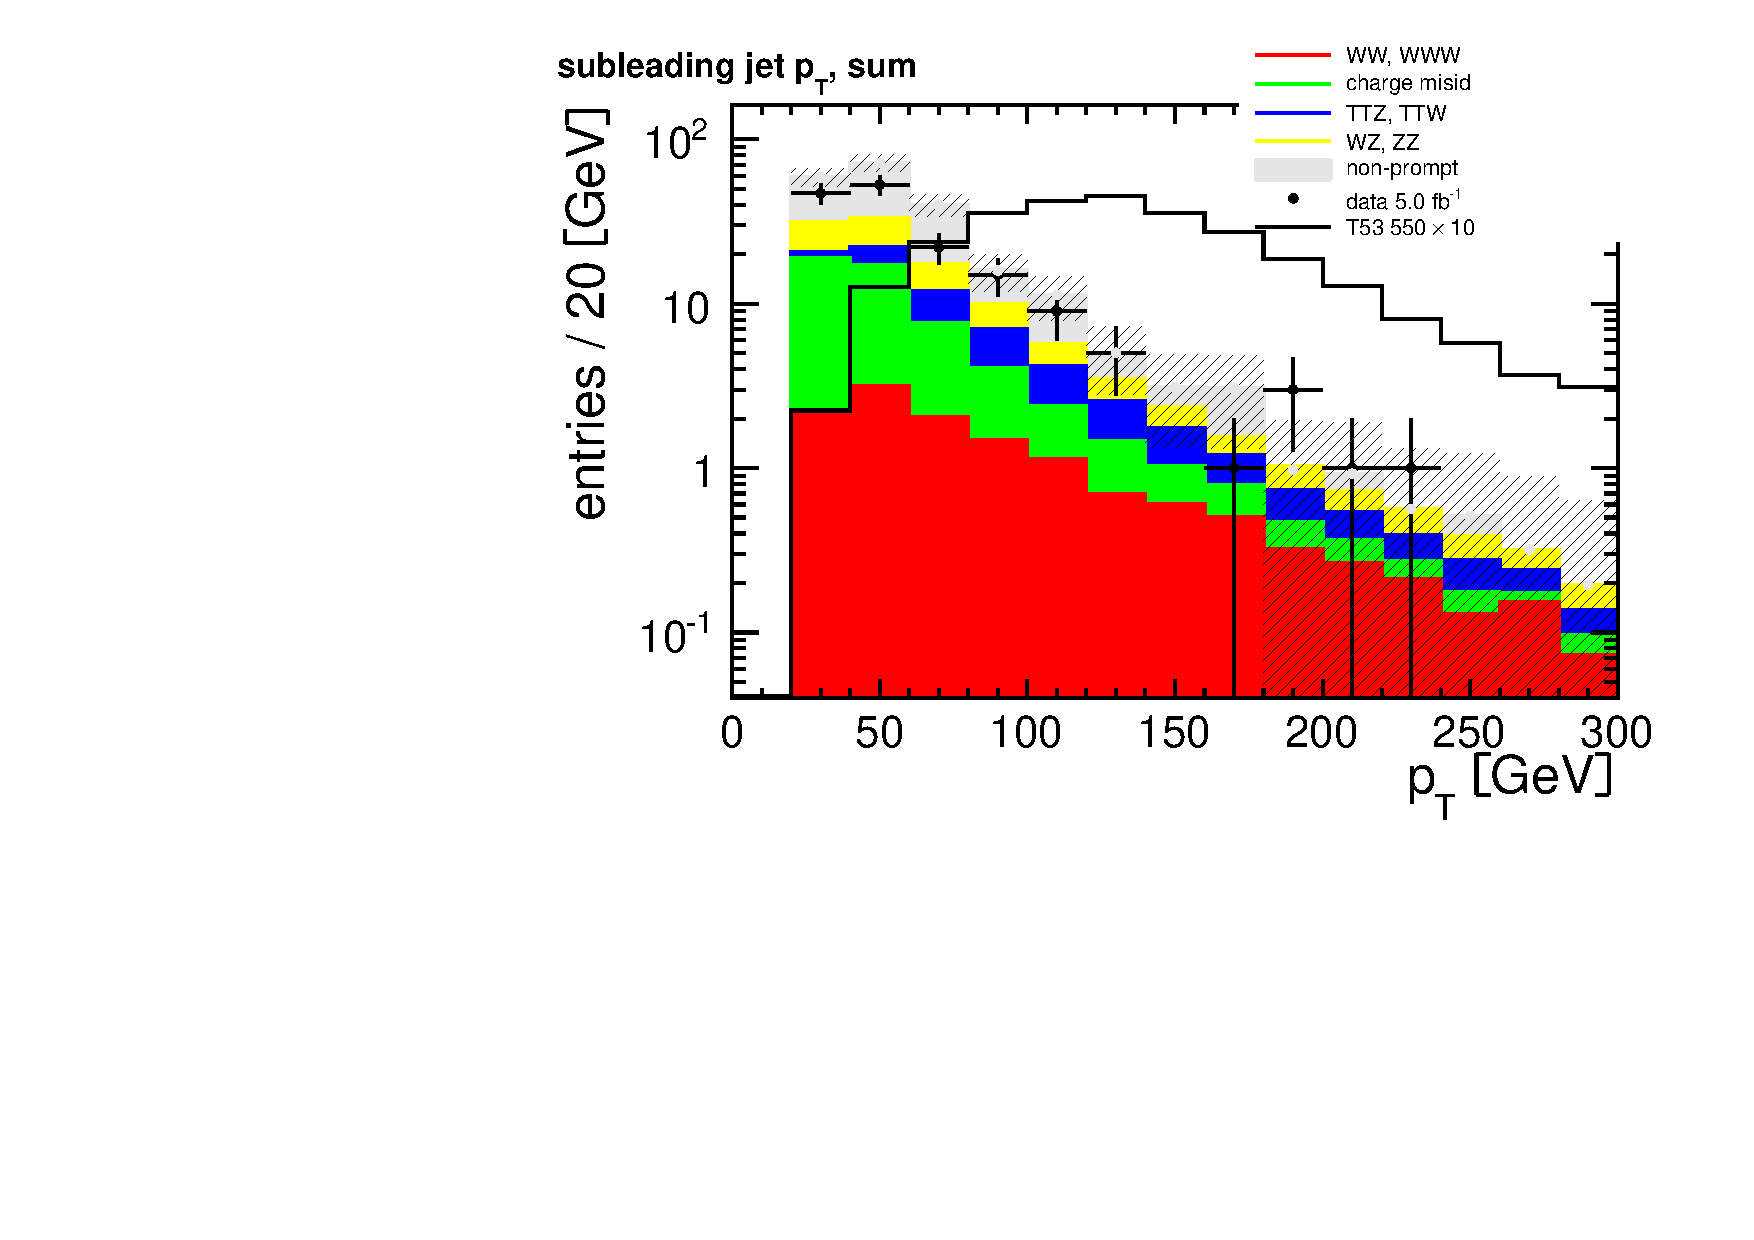
\includegraphics[width=.7\textwidth]{images/pdf/same-sign,_2_jets/jet_pt_2_sum_1}
    \caption{Expected and observed distributions of the \pt of the leading
    (top) and subleading (bottom) jet in events with two same-sign leptons
and two jets. The sum of the three decay channels is shown. }
    \label{fig:jet_pt}
\end{figure}

\begin{figure}[htb]
    \centering
    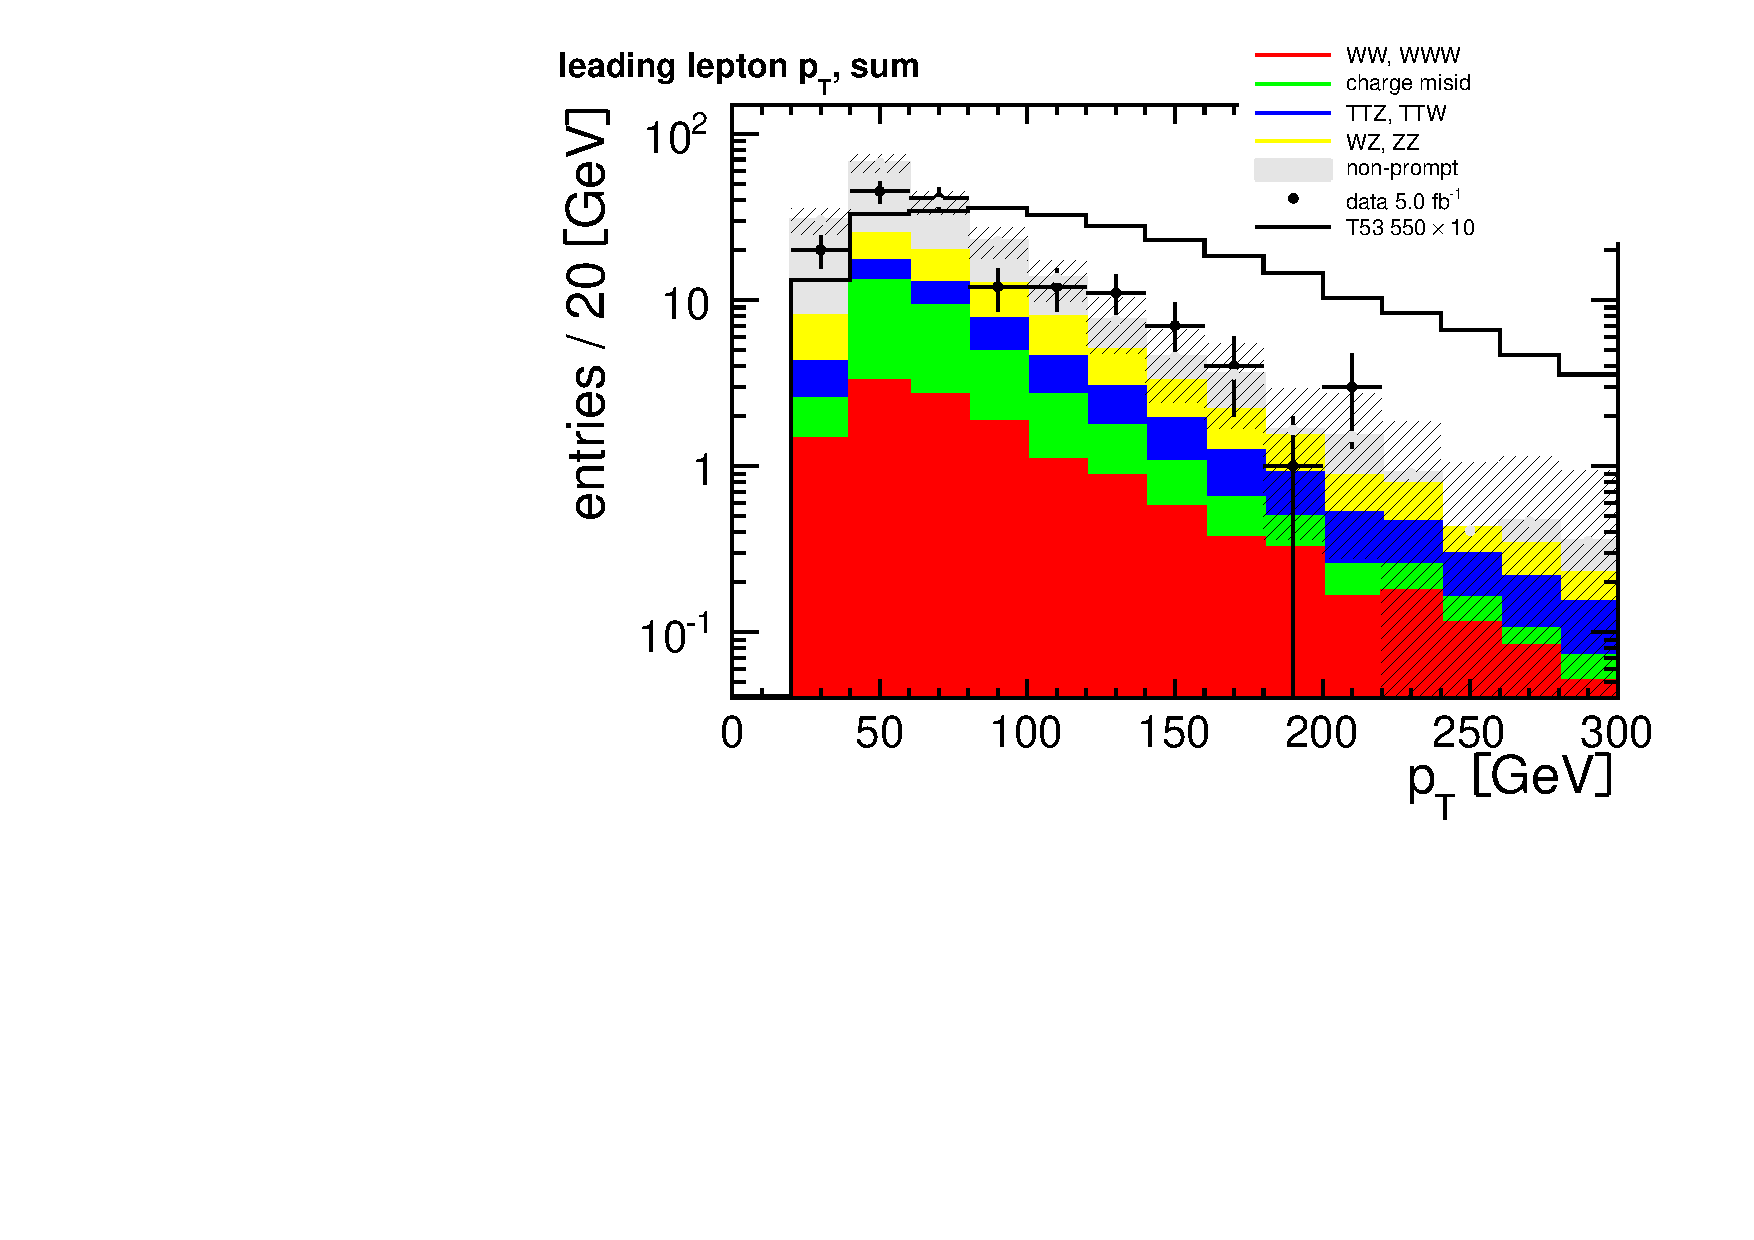
\includegraphics[width=.7\textwidth]{images/pdf/same-sign,_2_jets/lep_pt_1_sum_1}\\
    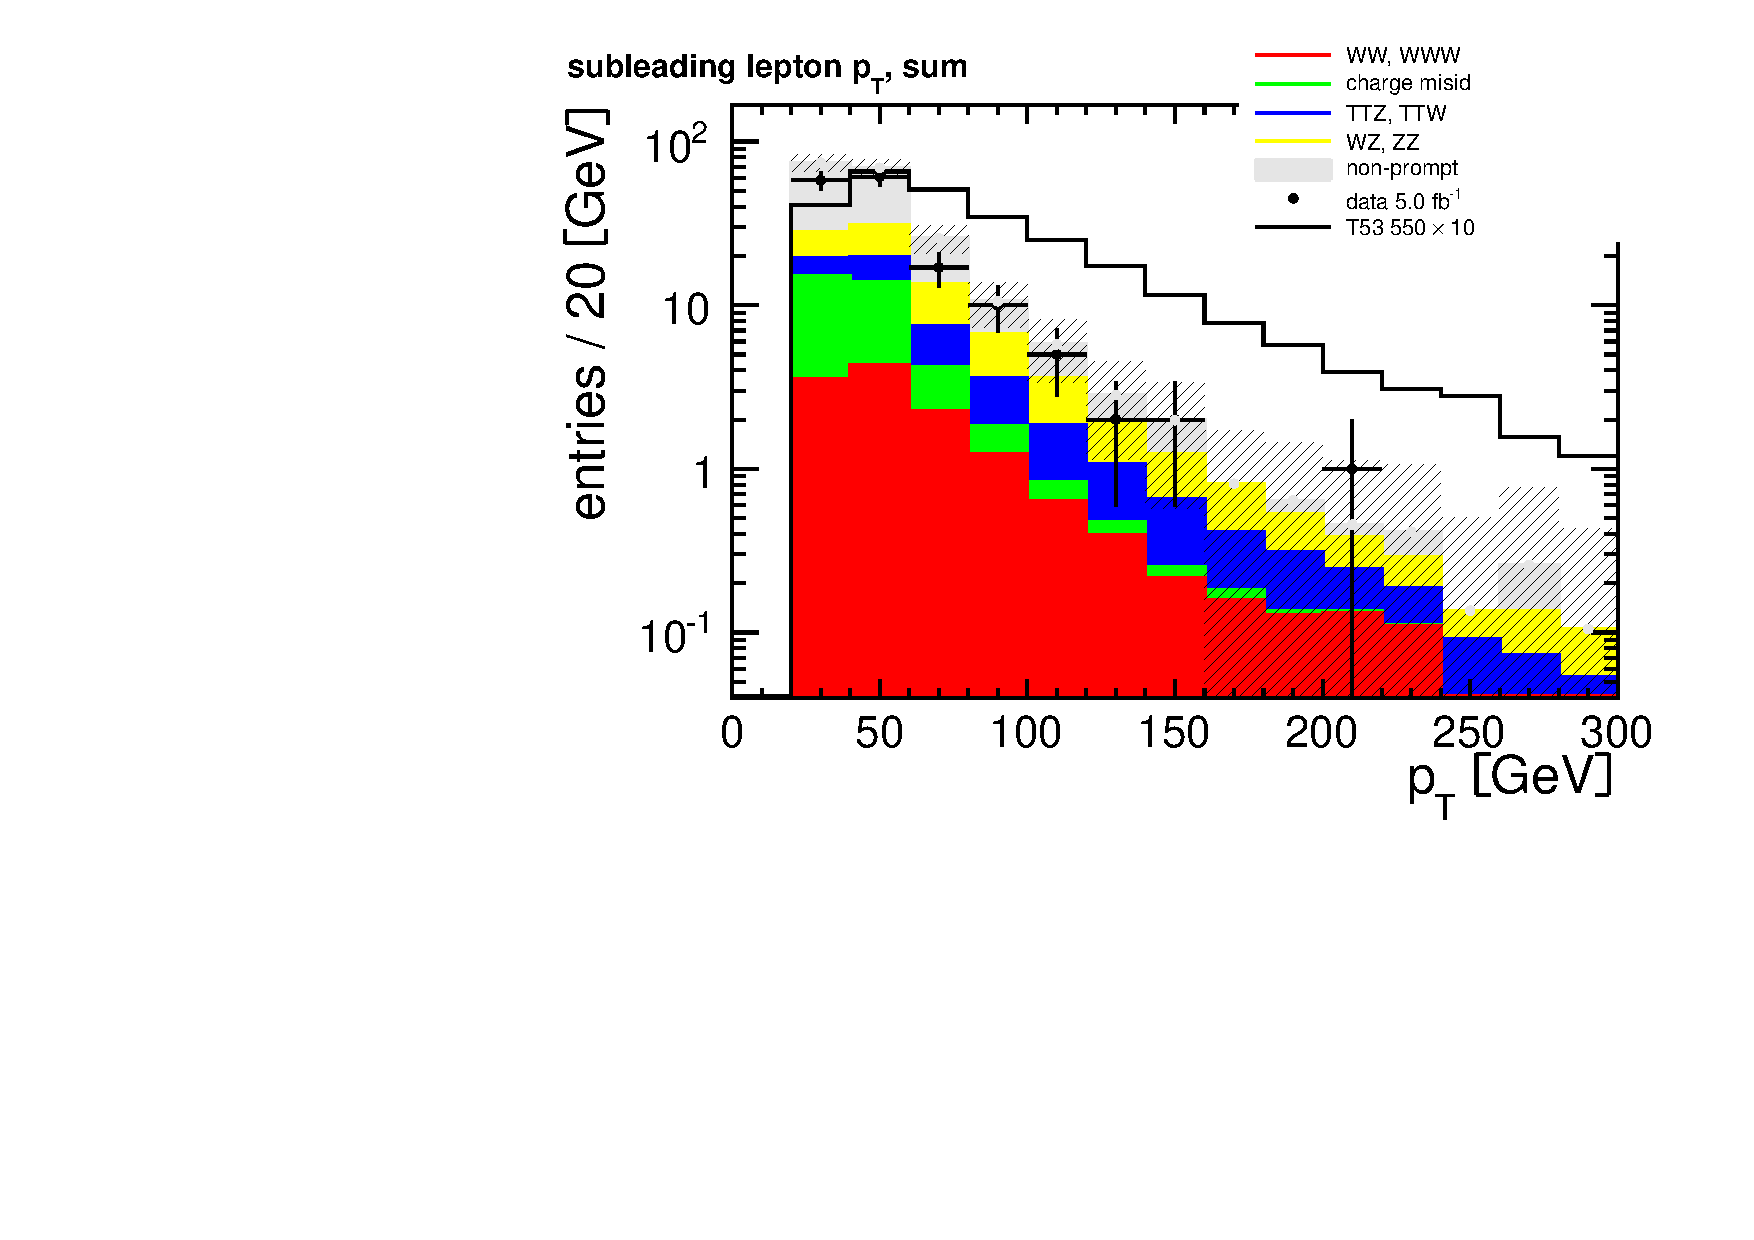
\includegraphics[width=.7\textwidth]{images/pdf/same-sign,_2_jets/lep_pt_2_sum_1}
    \caption{Expected and observed distributions of the \pt of the leading
    (top) and subleading (bottom) leptons in events with two same-sign leptons
and two jets. The sum of the three decay channels is shown. }
    \label{fig:lep_pt}
\end{figure}

\begin{figure}[htb]
    \centering
    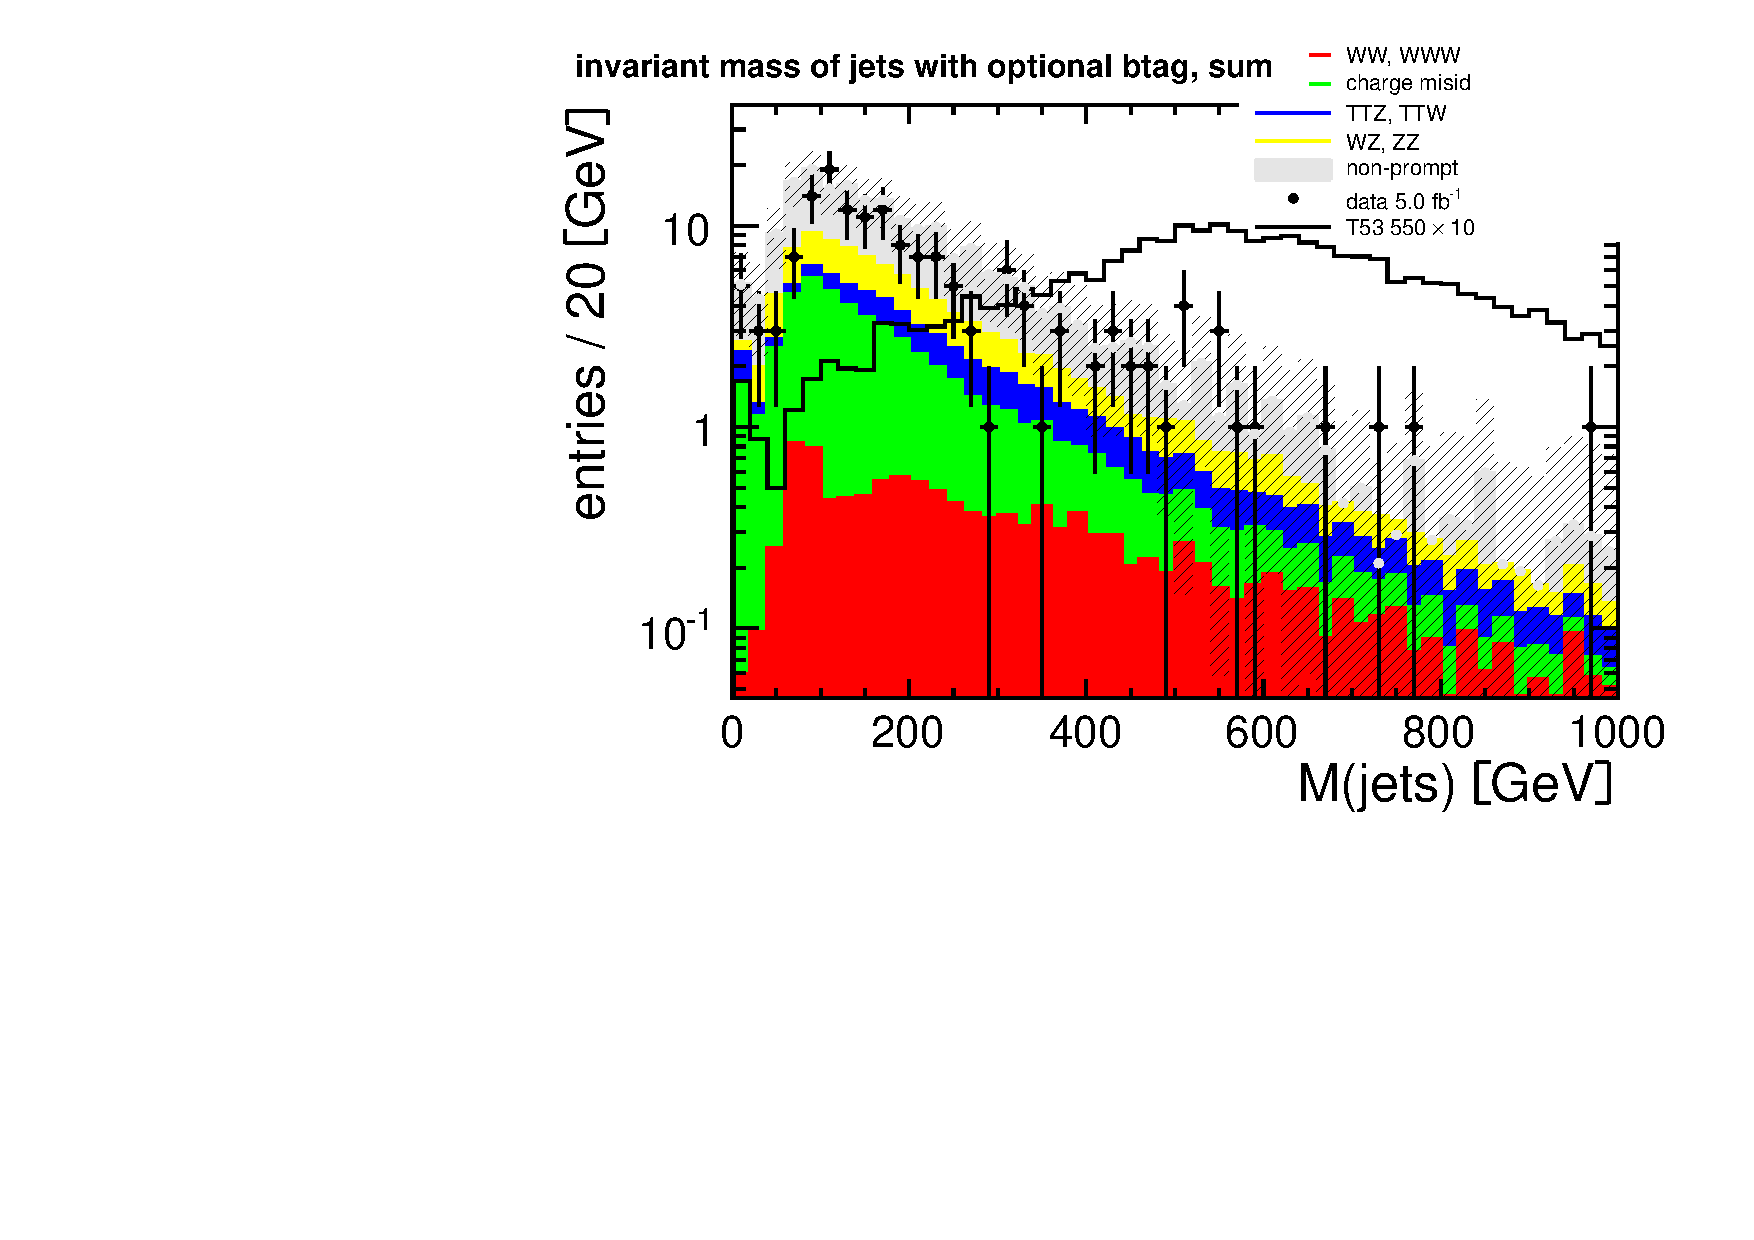
\includegraphics[width=.7\textwidth]{images/pdf/same-sign,_2_jets/had_mass_optional_btag_sum_1}\\
    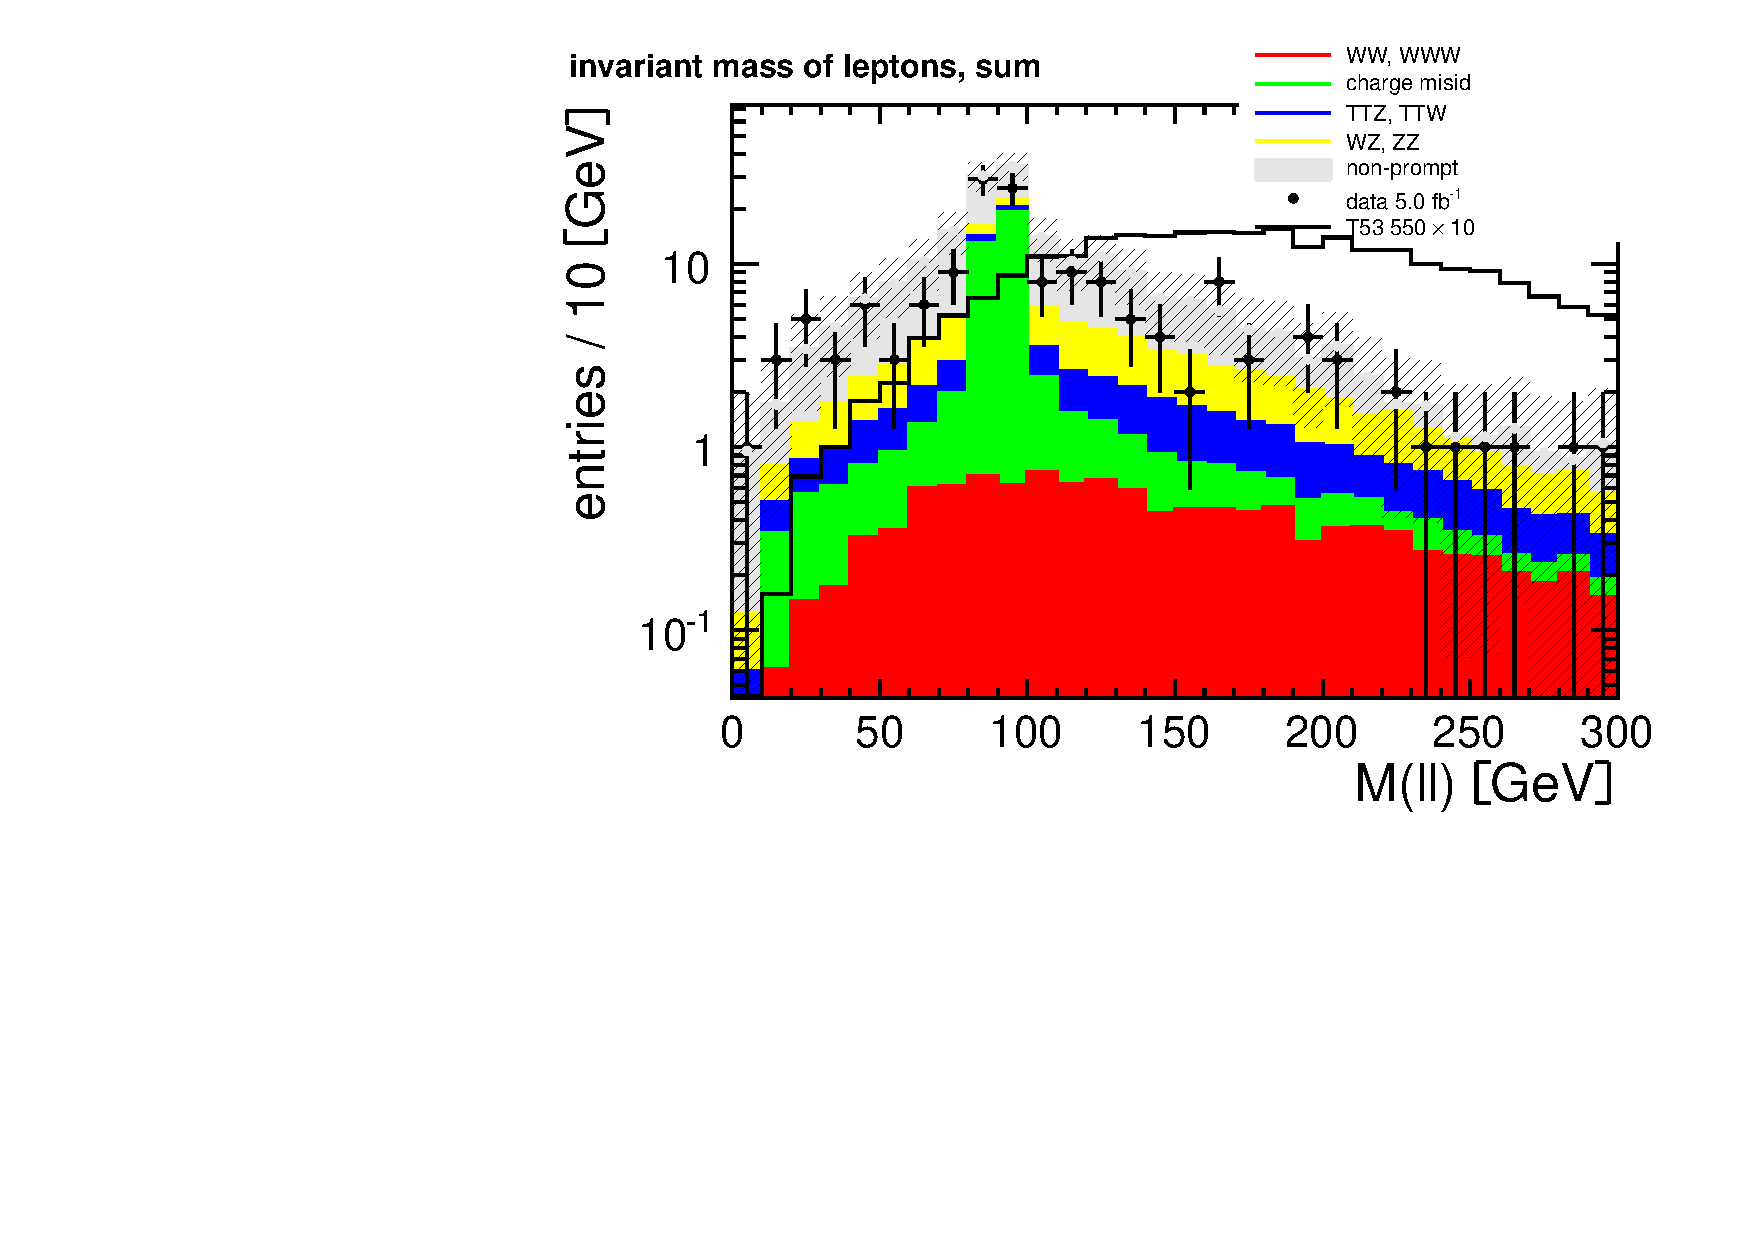
\includegraphics[width=.7\textwidth]{images/pdf/same-sign,_2_jets/lep_mass_sum_1}
    \caption{Expected and observed distributions of the invariant mass of
        jets (top) and leptons (bottom) in events with two same-sign leptons
        and two jets. The sum of the three decay channels is shown. The \emph{optional b-tag} method for calculating the
        invariant mass of the jets is described in~\ref{sec:razor_btagging}.}
    \label{fig:masses}
\end{figure}
